% Created 2010-08-17 Tue 13:49
\documentclass{article}
\usepackage{graphicx}
\usepackage{times}
\usepackage[margin=0.75in]{geometry}


\title{Inserting an AHIR module in the NetFPGA framework}
\author{Madhav Desai}

\begin{document}

\maketitle

\section{Overview}

This document describes the mechanism by which an 
AHIR generated VHDL system can be included in the NetFPGA packet
processing implementation framework.  

The AHIR generated VHDL system is required to fit into 
a NetFPGA user-module template (described below).  Thus,
the AHIR generated VHDL system must be wrapped into
a form expected by the NetFPGA user-module template.

\section{Mechanism}

The user module template has the form (the original
NetFPGA module is in Verilog; we use a VHDL equivalent).
\begin{verbatim}
entity module_template is
   generic (
      DATA_WIDTH: integer := 64;
      CTR_WIDTH: integer := 8;
      UDP_REG_SRC_WIDTH: integer := 2
   );
   port (
      in_data: in std_logic_vector(DATA_WIDTH-1 downto 0);
      in_ctrl: in std_logic_vector(CTRL_WIDTH-1 downto 0);
      in_wr: in std_logic;
      in_rdy: out std_logic;

      out_data: out std_logic_vector(DATA_WIDTH-1 downto 0);
      out_ctrl: out std_logic_vector(CTRL_WIDTH-1 downto 0);
      out_wr: out std_logic;
      out_rdy: in std_logic;

      clk: in std_logic;
      reset: in std_logic);
end entity;
\end{verbatim}
Thus, the NetFPGA user-module template can be viewed
as a system with a single input queue and a single output queue.

The AHIR system has form:
\begin{verbatim}
entity ahir_system is
   port(
          -- for each top-level function 
          --   (in this case int foo(int a))
          foo_a : in std_logic_vector(31 downto 0); -- argument a
          foo_ret_val_x_X: out std_logic_vector(31 downto 0); -- ret value
          foo_start: in std_logic;  -- pulse to start.
          foo_fin: out std_logic;   -- pulsed to indicate finish.
         
          -- for each input pipe
          --   (in this case inpipe of type int)
          inpipe_pipe_write_data: in std_logic_vector(31 downto 0); -- data
          inpipe_pipe_write_req: in std_logic_vector(0 downto 0); -- ready-in
          inpipe_pipe_write_ack: out std_logic_vector(0 downto 0); -- ready-ack.

          -- for each output pipe
          --   (in this case outpipe of type int)
          outpipe_pipe_read_data: out std_logic_vector(31 downto 0); -- data
          outpipe_pipe_read_req: in std_logic_vector(0 downto 0); -- ready-in
          outpipe_pipe_read_ack: out std_logic_vector(0 downto 0); -- ready-ack.

          clk: in std_logic;
          reset: in std_logic;
       );
end entity;
\end{verbatim}
An AHIR system can thus be viewed as having
\begin{itemize}
\item An input queue for each top-level function.
\item An output queue for each top-level function.
\item An input queue for each input pipe.
\item An output queue for each output pipe.
\end{itemize}


Thus, in order to insert an AHIR system into a NetFPGA user-module template,
all we need to do is
\begin{itemize}
\item Include an input-module which will collect data from the NetFPGA user-module
input data interface.  This input-module will feed the AHIR system input queues.
\begin{itemize}
\item This is especially simple if the AHIR system consists of a single top-level
function without pipes, since there is only one possible destination for the
incoming data.
\end{itemize}
\item Include an output-module which will collect data from the AHIR system
output queues
and forward it out of the output data interface of the NetFPGA user-module.
\begin{itemize}
\item Especially easy if there is only one top-level function in the AHIR
system without output pipes.
\end{itemize}
\item  In the general case (many top-level AHIR functions, with input and output
pipes), we will have to implement some kind of distributor/concentrator to
stream the data consistently between the NetFPGA user-module
input/output queues and the AHIR system input/output queues.
\end{itemize}

\section{Looking Ahead: a proposal for rapid deployment}

The process of including the AHIR system in a NetFPGA user template is
exactly the same as that of verifying an AHIR system using a C-testbench
with the assumption that the testbench only sends/receives packets to the AHIR 
system.  Most of the basic infrastructure for this is in place.  The only
necessary components are the input and output modules outlined in the 
previous section.

There could be three approaches:
\begin{itemize}
\item The input and output modules are written as VHDL modules with
adequate parametrization.  This should work if the AHIR system is
simple enough (consists of a system with a single top-level function
without any input/output pipes, for example).  However, writing
VHDL (or Verilog) implementations is a pain for more complex scenarios.
\item The input and output modules are written as C functions and
are included into the AHIR system.  This gives much more flexibility.
However, in a complex AHIR system, this approach will limit the
ability to exploit parallelism (note: we cannot use threads in these
C functions because AhirV2 tools cannot handle threads yet).
\item The input and output modules are written as Aa modules.  This
gives not only flexibility, but also the ability to use the
parallelism in the system.
\end{itemize}

Originally, Sameer had implemented the input and output module for
a specific scenario (as documented in the previous plan).  In this
scenario, the input module would receive the data from the NetFPGA
surroundings, would put the data packet into memory and would trigger
the AHIR module.  On completion of the AHIR module, the output module
would take the modified data from memory and would forward it to
the NetFPGA environment.   I have looked at the code and it
seems reasonably clean (will probably have to redo parts of it
to fit into the new AhirV2 scheme). 

What would be easiest, in my opinion would be
\begin{itemize}
\item Use the parts of Sameer's code that do the protocol
translation (between the NetFPGA user-module and an AHIR module).
\item Write the input and output modules in Aa.  For the moment,
we would do so for a specific scenario (much faster to develop and
easier to maintain).  This would remove the need to do memory 
management from the VHDL interface code (as is done in Sameer's
current implementation, in which the VHDL input module directly
accesses AHIR memory).
\item Generate the final AHIR system by including the input/output modules
written in Aa.
\item Instantiate the final AHIR system in a NetFPGA wrapper which 
just does the protocol translation between NetFPGA and AHIR.
\end{itemize}
This is indicated in Figure \ref{fig:Wrap}.   The only
additional effort is to write the input and output modules
and to write the wrap functionality in vc2vhdl.  This should
take a week.

\begin{figure}[!t]
  \centering
  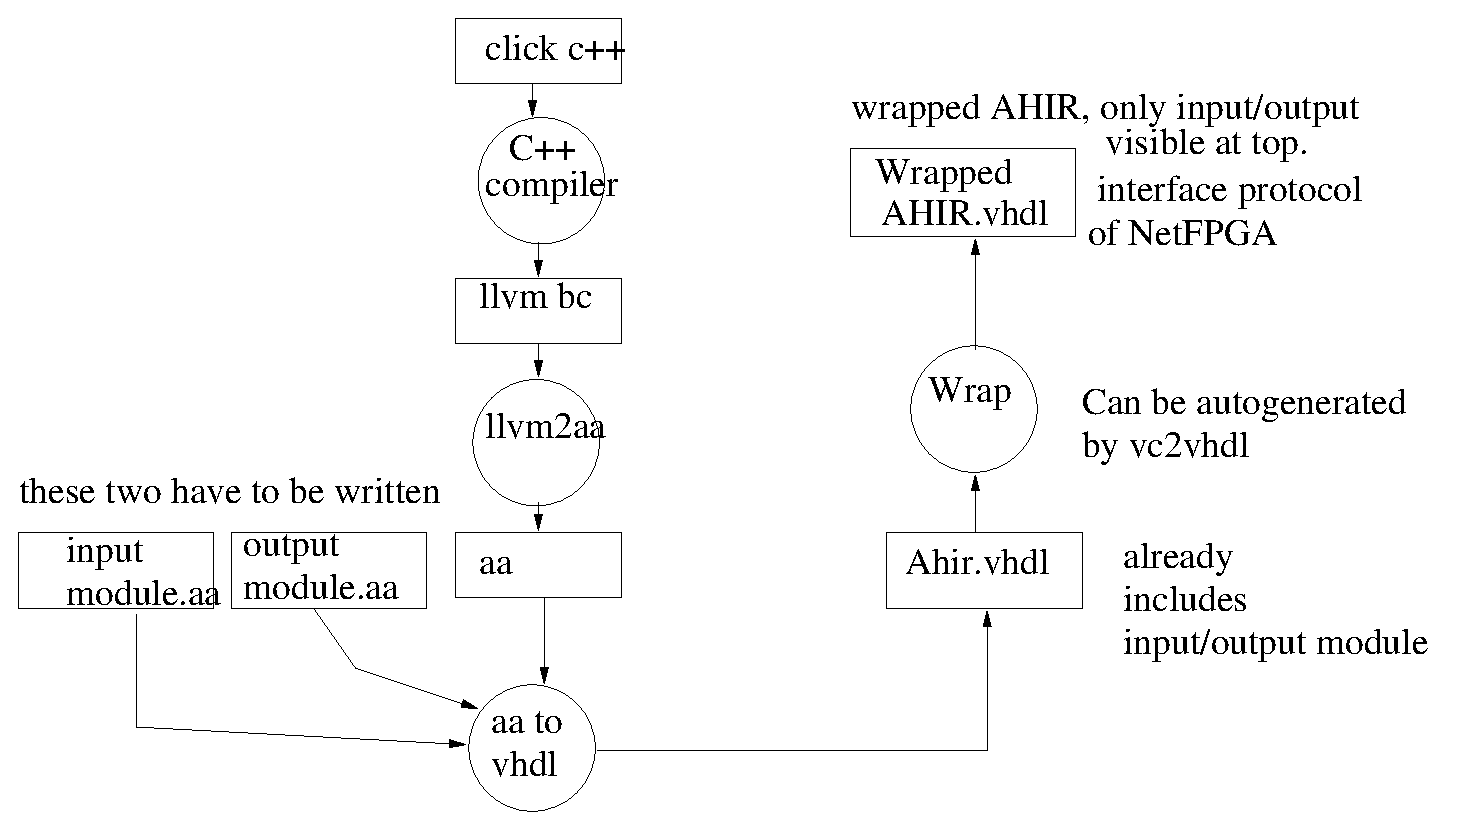
\includegraphics[scale=0.7]{NetFPGAWrap.eps}
  \caption{NetFPGA Wrap Flow}
  \label{fig:Wrap}
\end{figure}


\end{document}
